\documentclass[12pt,border=6pt]{standalone}
\usepackage{fontspec}
\setmainfont{BeVietnamPro}[Path=D:/IOT_Tools/downloads/fonts/,Extension=.ttf,UprightFont=*-Regular,BoldFont=*-Bold]
\usepackage{amsmath}
\usepackage{unicode-math}\setmathfont{Cambria Math}
\usepackage{xcolor}
\usepackage{tikz}
\usetikzlibrary{positioning,arrows.meta,shapes.geometric,shapes.misc,calc,fit,backgrounds,decorations.pathreplacing,shadows,3d,perspective}
\usepackage{tikz-3dplot}
\usepackage{pgfplots}\pgfplotsset{compat=1.18}
\usepgfplotslibrary{groupplots,fillbetween}
\definecolor{cDo}{HTML}{BB2025}\definecolor{cDoD}{HTML}{8E1418}\definecolor{cDoT}{HTML}{FCEBEC}
\definecolor{cXanh}{HTML}{326CE5}\definecolor{cXanhT}{HTML}{EAF0FC}
\definecolor{cLuc}{HTML}{15803D}\definecolor{cLucT}{HTML}{E6F4EA}
\definecolor{cVang}{HTML}{B45309}\definecolor{cVangT}{HTML}{FDF2E1}
\definecolor{cNavy}{HTML}{1E293B}\definecolor{cMuc}{HTML}{1F2937}\definecolor{cXam}{HTML}{4B5563}
\definecolor{cXamT}{HTML}{F3F4F6}\definecolor{cVien}{HTML}{DDE1E6}\definecolor{cTim}{HTML}{6D28D9}\definecolor{cTimT}{HTML}{F1EBFD}
\pgfplotsset{slide/.style={tick label style={font=\small}, label style={font=\small}, scaled ticks=false,
  /pgf/number format/fixed, /pgf/number format/use comma, /pgf/number format/1000 sep={\,},
  legend style={font=\small,draw=none,fill=none}, axis line style={cXam}, major tick style={cXam},
  grid style={cVien}}}
\pgfkeys{/pgf/number format/assume math mode=true}
\begin{document}
% F03 · S04 · kiến trúc hệ thống (chiếu isometric): drone (FC, ESC, GPS, TFmini, bộ thu, ESP32 DroneBridge, camera ESP32-S3),
% hotspot IOTCV-HOTSPOT 2,4 GHz, laptop (backend FastAPI :8000 + AI ONNX GPU), trình duyệt (web :5173), tay phát FS-i6X.
% Nguồn: facts/03-phan-mem.md mục 1 (chay-drone-that.bat, backend/config.py dòng 102 đến 105); facts/01-phan-cung.md mục 2;
% facts/02-firmware-cau-hinh.md mục 3, 7, 8. Khung slide 12,6 x 8,8 in; vẽ đúng cỡ in, chữ nhỏ nhất 15 pt.
\newfontfamily\monof{Consolas}%
\newfontface\semib{BeVietnamPro-SemiBold}[Path=D:/IOT_Tools/downloads/fonts/,Extension=.ttf]%
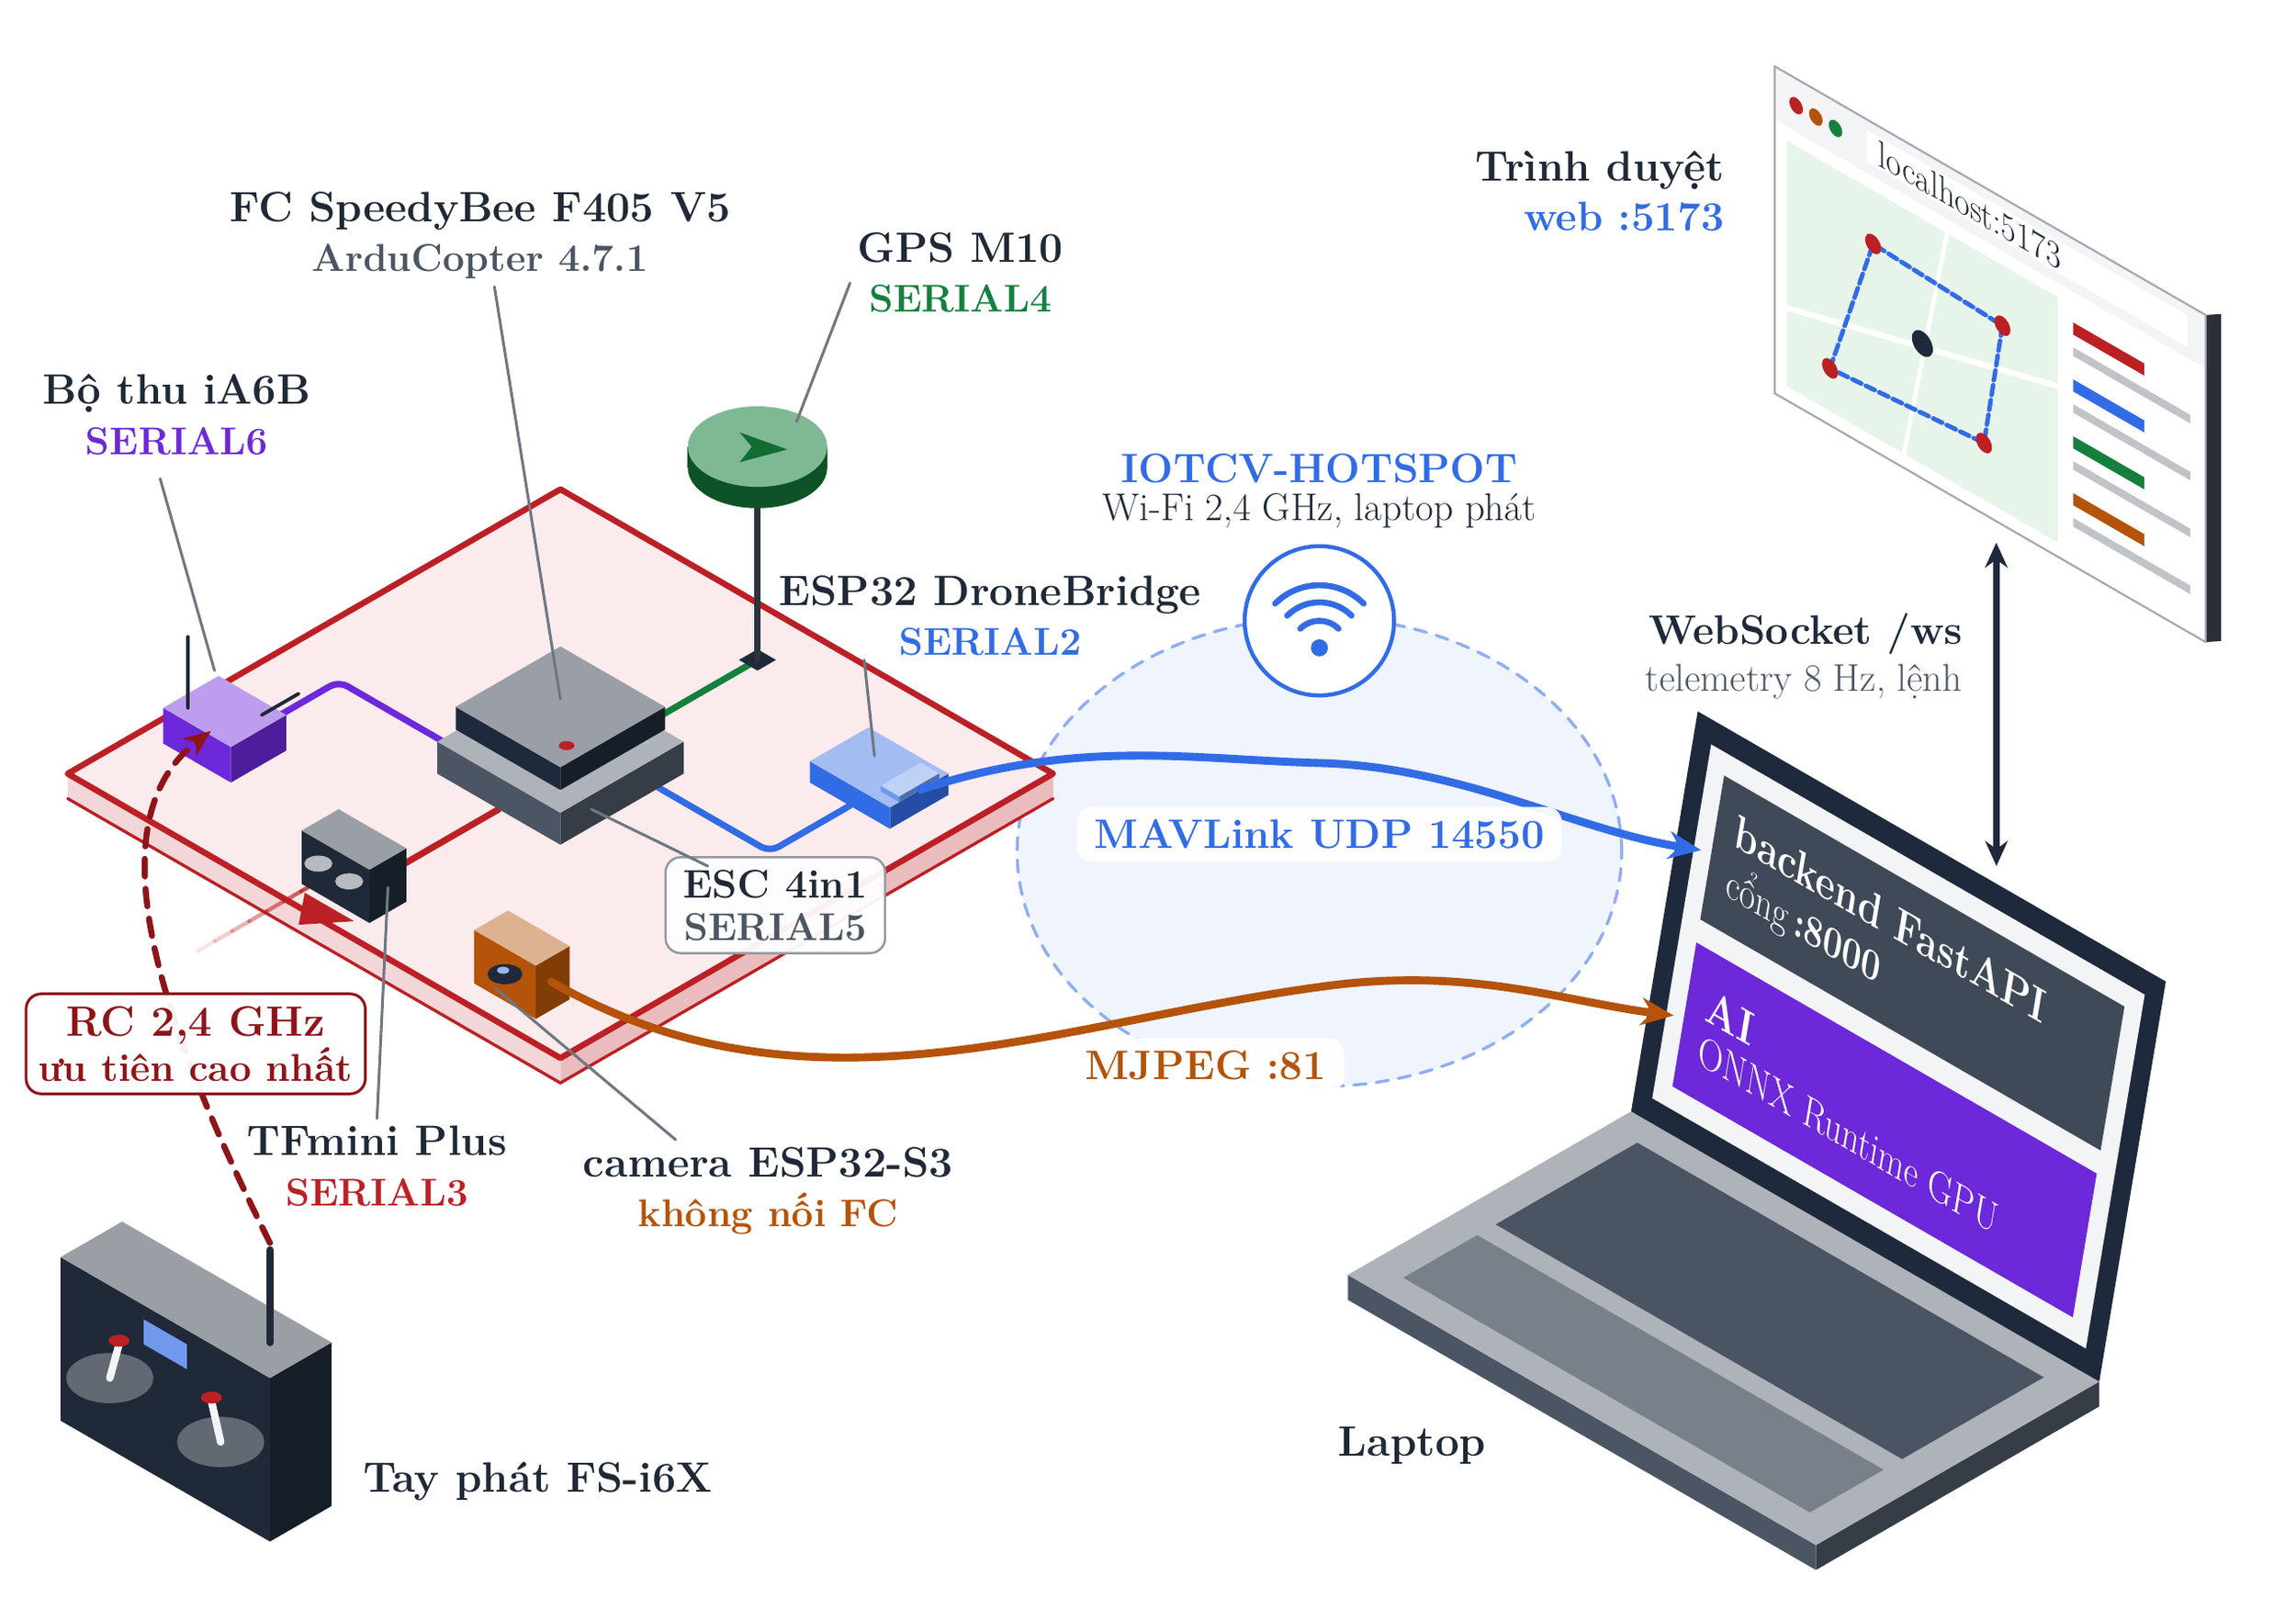
\begin{tikzpicture}[line join=round,line cap=round,
  iso/.style={x={(0.866cm,-0.5cm)},y={(0.866cm,0.5cm)},z={(0cm,1cm)}},
  nm/.style={font=\fontsize{17}{19}\bfseries,text=cMuc,inner sep=0pt,align=center},
  tag/.style={fill=white,fill opacity=.94,text opacity=1,rounded corners=6pt,inner xsep=7pt,inner ysep=5pt,align=center},
  ld/.style={line width=1.1pt,cXam!80!white}]
\frenchspacing
\useasboundingbox (0,0) rectangle (31.57,21.93);
% hộp isometric: thấy mặt +x (tối), -y (vừa), +z (sáng)
\newcommand\ibox[7]{%
  \fill[#7!72!black] (#1+#4,#2,#3) -- (#1+#4,#2+#5,#3) -- (#1+#4,#2+#5,#3+#6) -- (#1+#4,#2,#3+#6) -- cycle;
  \fill[#7] (#1,#2,#3) -- (#1+#4,#2,#3) -- (#1+#4,#2,#3+#6) -- (#1,#2,#3+#6) -- cycle;
  \fill[#7!45!white] (#1,#2,#3+#6) -- (#1+#4,#2,#3+#6) -- (#1+#4,#2+#5,#3+#6) -- (#1,#2+#5,#3+#6) -- cycle;}
\newcommand\qd[4]{(#1,#2) -- (#3,#2) -- (#3,#4) -- (#1,#4) -- cycle}
\newcommand\ptf{\monof\bfseries\fontsize{15.5}{18}\selectfont}
\newcommand\sbf{\semib\fontsize{15.5}{18}\selectfont}
% ================= vùng Wi-Fi của hotspot (nền)
\fill[cXanhT,opacity=.75] (18.2,10.3) ellipse (4.25 and 3.3);
\draw[cXanh!55,line width=1.2pt,dash pattern=on 5pt off 4pt] (18.2,10.3) ellipse (4.25 and 3.3);
% ================= DRONE: tấm nền nghiêng 8 x 8, mũi = phía -y (mép trái dưới)
\begin{scope}[shift={(0.6,11.4)},iso]
  \fill[cDo!30!white] (8,0,-0.35) -- (8,8,-0.35) -- (8,8,0) -- (8,0,0) -- cycle;
  \fill[cDo!18!white] (0,0,-0.35) -- (8,0,-0.35) -- (8,0,0) -- (0,0,0) -- cycle;
  \fill[cDoT] (0,0,0) -- (8,0,0) -- (8,8,0) -- (0,8,0) -- cycle;
  \draw[cDo,line width=2.4pt] (0,0,0) -- (8,0,0) -- (8,8,0) -- (0,8,0) -- cycle;
  \draw[cDo,line width=1.2pt] (0,0,-0.35) -- (8,0,-0.35) -- (8,8,-0.35);
  \fill[cDo] (4.0,-0.25,0) -- (3.6,0.25,0) -- (4.4,0.25,0) -- cycle;
  % dây UART trên mặt nền
  \draw[cXanh,line width=2.6pt,rounded corners=4pt] (5.0,4.6,0) -- (6.8,4.6,0) -- (6.8,5.9,0);
  \draw[cDo,line width=2.6pt] (4.0,3.0,0) -- (4.0,0.95,0);
  \draw[cLuc,line width=2.6pt] (4.0,5.0,0) -- (4.0,7.1,0);
  \draw[cTim,line width=2.6pt,rounded corners=4pt] (3.0,3.5,0) -- (0.9,3.5,0) -- (0.9,2.1,0);
  % bộ thu iA6B + 2 anten
  \ibox{0.35}{1.2}{0}{1.1}{0.9}{0.5}{cTim}
  \draw[cMuc,line width=1.4pt] (0.55,1.4,0.5) -- (0.55,1.4,1.5);
  \draw[cMuc,line width=1.4pt] (1.25,1.9,0.5) -- (1.85,1.9,1.1);
  \coordinate (rx) at (0.9,1.6,0.6);
  % GPS: cột ở đuôi
  \fill[cMuc] (3.85,7.05,0) -- (4.15,7.05,0) -- (4.15,7.35,0) -- (3.85,7.35,0) -- cycle;
  \draw[cXam!60!black,line width=2.6pt] (4.0,7.2,0) -- (4.0,7.2,2.7);
  \coordinate (gpsb) at (4.0,7.2,2.7);\coordinate (gpst) at (4.0,7.2,3.0);
  % ESC 4in1 + FC (stack)
  \ibox{3.0}{3.0}{0}{2.0}{2.0}{0.45}{cXam}
  \foreach \px/\py in {3.3/3.3,4.7/3.3,4.7/4.7} \draw[cXam!40!white,line width=1.6pt] (\px,\py,0.45) -- (\px,\py,0.62);
  \ibox{3.15}{3.15}{0.62}{1.7}{1.7}{0.32}{cNavy}
  \fill[cDo] (4.6,3.5,0.945) circle (0.09);
  \coordinate (fc) at (3.9,4.1,0.95);\coordinate (esc) at (5.0,3.5,0.25);
  % ESP32 DroneBridge
  \ibox{6.15}{5.9}{0}{1.3}{0.95}{0.3}{cXanh}
  \ibox{7.15}{6.05}{0.3}{0.3}{0.65}{0.08}{cXanh!70!white}
  \coordinate (db) at (6.6,6.5,0.3);\coordinate (dbw) at (7.45,6.4,0.3);
  % TFmini ở mũi + tia
  \foreach \i in {0,...,7}{\pgfmathsetmacro\op{0.9*(1-\i/8)}
    \draw[cDo,opacity=\op,line width=1.6pt] (4.0,{0.35-0.28*\i},0.45) -- (4.0,{0.35-0.28*(\i+1)},0.45);}
  \ibox{3.45}{0.35}{0}{1.1}{0.6}{0.75}{cMuc}
  \fill[cXam!40!white] (3.72,0.35,0.42) circle (0.16);\fill[cXam!40!white] (4.22,0.35,0.42) circle (0.16);
  \coordinate (tf) at (4.55,0.65,0.35);
  % camera ESP32-S3 (mép trước, gần góc dưới)
  \ibox{6.25}{0.35}{0}{1.0}{0.55}{0.75}{cVang}
  \fill[cMuc] (6.75,0.35,0.38) circle (0.2);\fill[cXanh!50!white] (6.72,0.35,0.42) circle (0.07);
  \coordinate (cam) at (7.25,0.6,0.4);\coordinate (camL) at (6.6,0.35,0.1);
\end{scope}
% đĩa GPS (trụ, toạ độ giấy)
\fill[cLuc!65!black] ($(gpsb)+(-0.98,0)$) rectangle ($(gpst)+(0.98,0)$);
\fill[cLuc!65!black] (gpsb) ellipse (0.98 and 0.566);
\fill[cLuc!55!white] (gpst) ellipse (0.98 and 0.566);
\fill[cLuc!85!black] ($(gpst)+(0.42,-0.04)$) -- ($(gpst)+(-0.25,0.2)$) -- ($(gpst)+(-0.08,0)$) -- ($(gpst)+(-0.25,-0.22)$) -- cycle;
% ================= RC FS-i6X (góc trái dưới)
\begin{scope}[shift={(0.5,2.3)},iso]
  \ibox{0}{0}{0}{3.4}{1.0}{2.3}{cMuc}
  \fill[cMuc!70!white] (0.8,0,1.0) circle (0.5);\fill[cMuc!70!white] (2.6,0,1.0) circle (0.5);
  \draw[cXamT,line width=3pt] (0.8,0,1.0) -- (0.95,0,1.55);\fill[cDo] (0.95,0,1.6) circle (0.12);
  \draw[cXamT,line width=3pt] (2.6,0,1.0) -- (2.45,0,1.5);\fill[cDo] (2.45,0,1.55) circle (0.12);
  \fill[cXanh!70!white] (1.35,0,1.75) -- (2.05,0,1.75) -- (2.05,0,2.1) -- (1.35,0,2.1) -- cycle;
  \draw[cMuc,line width=3pt] (2.9,0.5,2.3) -- (2.9,0.5,3.6);
  \coordinate (rca) at (2.9,0.5,3.7);
\end{scope}
\node[nm,anchor=west] at (4.75,1.45) {Tay phát FS-i6X};
% đường RC 2,4 GHz (đỏ đậm, nét đứt) tới bộ thu
\draw[cDoD,line width=2.4pt,dash pattern=on 7pt off 5pt,-{Stealth[length=11pt,width=9pt]}]
  (rca) .. controls ($(rca)+(-1.6,3.2)$) and ($(rx)+(-1.8,-1.6)$) .. ($(rx)+(-0.15,-0.35)$);
\node[tag,inner xsep=5pt,text=cDoD,font=\fontsize{17}{19}\bfseries,draw=cDoD,line width=1.1pt] at (2.4,7.6)
  {RC 2,4 GHz\\[-1pt]{\sbf ưu tiên cao nhất}};
% ================= laptop (đế 7,6 x 4,6 + màn hình ngả 12°)
\begin{scope}[shift={(18.6,4.0)},iso]
  \ibox{0}{0}{0}{7.6}{4.6}{0.35}{cXam}
  \fill[cXam!75!white] (0.5,0.4,0.36) -- (7.1,0.4,0.36) -- (7.1,1.6,0.36) -- (0.5,1.6,0.36) -- cycle;
  \fill[cNavy!80!white] (0.5,1.9,0.36) -- (7.1,1.9,0.36) -- (7.1,4.2,0.36) -- (0.5,4.2,0.36) -- cycle;
  \coordinate (scr) at (0,4.6,0.35);
\end{scope}
\begin{scope}[cm={0.866,-0.5,0.18,1.082,(scr)}]
  \fill[cNavy] \qd{0}{0}{7.6}{5.2};
  \fill[cXamT] \qd{0.28}{0.3}{7.32}{4.9};
  \fill[cNavy!85!white] \qd{0.55}{2.75}{7.05}{4.62};
  \fill[cTim] \qd{0.55}{0.58}{7.05}{2.45};
  \node[transform shape,text=white,anchor=west,inner sep=0pt,align=left] at (0.85,3.68)
    {{\fontsize{17}{19}\bfseries backend FastAPI}\\[4pt]{\semib\fontsize{15.5}{17}\selectfont cổng\,}{\monof\bfseries\fontsize{15.5}{17}\selectfont :8000}};
  \node[transform shape,text=white,anchor=west,inner sep=0pt,align=left] at (0.85,1.51)
    {{\fontsize{17}{19}\bfseries AI}\\[4pt]{\semib\fontsize{15.5}{17}\selectfont ONNX Runtime GPU}};
  \coordinate (be) at (0.55,3.65);\coordinate (ai) at (0.55,1.5);\coordinate (beT) at (4.85,5.2);
\end{scope}
\node[nm,anchor=east] at (20.55,1.95) {Laptop};
% ================= trình duyệt (cửa sổ đứng)
\begin{scope}[cm={0.866,-0.5,0,1,(24.6,16.75)}]
  \fill[cXam!55!black] (7,0) -- (7.25,0.14) -- (7.25,4.74) -- (7,4.6) -- cycle;
  \fill[white] \qd{0}{0}{7}{4.6};
  \fill[cXamT] \qd{0}{3.85}{7}{4.6};
  \foreach \i/\c in {0/cDo,1/cVang,2/cLuc} \fill[\c] ({0.35+0.32*\i},4.22) circle (0.11);
  \fill[white] \qd{1.5}{4.0}{6.7}{4.45};
  \node[transform shape,anchor=west,inner sep=0pt,text=cMuc,font=\monof\fontsize{15}{15}\selectfont] at (1.68,4.225) {localhost:5173};
  \fill[cLucT] \qd{0.2}{0.2}{4.6}{3.65};
  \draw[white,line width=2.4pt] (0.2,1.3) -- (4.6,2.4);
  \draw[white,line width=1.8pt] (2.1,0.2) -- (2.8,3.65);
  \draw[cXanh,line width=1.8pt,dash pattern=on 4pt off 2pt] (0.9,0.8) -- (1.6,2.9) -- (3.7,2.8) -- (3.4,1.0) -- cycle;
  \foreach \p in {(0.9,0.8),(1.6,2.9),(3.7,2.8),(3.4,1.0)} \fill[cDo] \p circle (0.13);
  \fill[cNavy] (2.4,1.9) circle (0.17);
  \foreach \i/\c in {0/cDo,1/cXanh,2/cLuc,3/cVang}{
    \fill[\c] \qd{4.85}{3.25-0.8*\i}{6.0}{3.42-0.8*\i};
    \fill[cXam!35!white] \qd{4.85}{2.95-0.8*\i}{6.75}{3.07-0.8*\i};}
  \draw[cXam!50!white,line width=0.8pt] \qd{0}{0}{7}{4.6};
  \coordinate (brB) at (3.6,0);
\end{scope}
\node[anchor=east,align=right,inner sep=0pt] at (23.9,19.6)
  {{\fontsize{17}{19}\bfseries\color{cMuc} Trình duyệt}\\[4pt]{\monof\bfseries\fontsize{16.5}{18}\selectfont\color{cXanh} web :5173}};
% backend ↔ web
\draw[cNavy,line width=2.6pt,{Stealth[length=10pt,width=9pt]}-{Stealth[length=10pt,width=9pt]}]
  ($(beT)+(0,0.25)$) -- ($(brB)+(0,-0.3)$);
\node[anchor=east,align=right,inner sep=0pt] at (27.25,13.05)
  {{\monof\bfseries\fontsize{16.5}{18}\selectfont\color{cNavy} WebSocket /ws}\\[3pt]{\sbf\color{cXam} telemetry 8 Hz, lệnh}};
% ================= hotspot
\coordinate (hs) at (18.2,13.55);
\fill[white] (hs) circle (1.05);\draw[cXanh,line width=1.6pt] (hs) circle (1.05);
\foreach \r in {0.38,0.64,0.88} \draw[cXanh,line width=2.4pt] ($(hs)+(45:\r)+(0,-0.38)$) arc[start angle=45,end angle=135,radius=\r];
\fill[cXanh] ($(hs)+(0,-0.38)$) circle (0.12);
\node[anchor=south,align=center,inner sep=0pt] at ($(hs)+(0,1.3)$)
  {{\monof\bfseries\fontsize{16.5}{18}\selectfont\color{cXanh} IOTCV-HOTSPOT}\\[3pt]{\sbf\color{cMuc} Wi-Fi 2,4 GHz, laptop phát}};
% ================= Wi-Fi: DroneBridge → backend (xanh), camera → AI (hổ phách), cùng đi qua hotspot
\draw[cXanh,line width=3.2pt,-{Stealth[length=13pt,width=11pt]}]
  (dbw) .. controls (14.8,11.9) and (16.4,11.6) .. (18.2,11.55) .. controls (20.2,11.5) and (21.8,10.6) .. ($(be)+(-0.15,0)$);
\draw[cVang,line width=3.2pt,-{Stealth[length=13pt,width=11pt]}]
  (cam) .. controls (11.0,6.4) and (14.5,7.9) .. (18.2,8.4) .. controls (20.3,8.7) and (21.6,8.2) .. ($(ai)+(-0.15,0)$);
\node[tag,text=cXanh,font=\monof\bfseries\fontsize{16.5}{18}\selectfont] at (18.2,10.55) {MAVLink UDP 14550};
\node[tag,text=cVang,font=\monof\bfseries\fontsize{16.5}{18}\selectfont] at (16.6,7.3) {MJPEG :81};
% ================= nhãn thiết bị trên drone
\node[nm,anchor=south] at (6.4,18.35) {FC SpeedyBee F405 V5\\[1pt]{\sbf\color{cXam} ArduCopter 4.7.1}};
\draw[ld] (6.6,18.25) -- (fc);
\node[nm,anchor=west] at (11.7,18.45) {GPS M10\\[1pt]{\ptf\color{cLuc} SERIAL4}};
\draw[ld] (11.6,18.3) -- ($(gpst)+(0.55,0.35)$);
\node[nm,anchor=west] at (0.25,16.45) {Bộ thu iA6B\\[1pt]{\ptf\color{cTim} SERIAL6}};
\draw[ld] (1.9,15.55) -- ($(rx)+(-0.1,0.5)$);
\node[nm,anchor=south west] at (10.6,13.05) {ESP32 DroneBridge\\[1pt]{\ptf\color{cXanh} SERIAL2}};
\draw[ld] (11.8,13.0) -- (db);
\node[nm,anchor=north] at (4.95,6.45) {TFmini Plus\\[1pt]{\ptf\color{cDo} SERIAL3}};
\draw[ld] (4.95,6.55) -- (tf);
\node[nm,anchor=north] at (10.45,6.15) {camera ESP32-S3\\[1pt]{\sbf\color{cVang} không nối FC}};
\draw[ld] (9.15,6.25) -- (camL);
\node[tag,draw=cXam!60,line width=0.9pt,font=\fontsize{16}{18}\bfseries,text=cMuc] at (10.55,9.55) {ESC 4in1\\[-1pt]{\ptf\color{cXam} SERIAL5}};
\draw[ld] (9.6,10.1) -- (esc);
\end{tikzpicture}

\end{document}
